\documentclass[11pt]{article}
\usepackage{aa}

\begin{document}
\zestaw{1}{Rekurencje typu „dziel i zwyciężaj”, twierdzenie o rekurencji uniwersalnej, drzewa rekursji}

\begin{teoria}[Jak czytać ten dokument]
Każde zadanie ma: przepisaną \textbf{treść} (szare pudełko), potrzebną
\textbf{teorię} (niebieskie), \textbf{intuicję} (żółte), \textbf{rozwiązanie
formalne} i~\textbf{odpowiedź} (zielone). Wyniki zostały sprawdzone
numerycznie skryptem \texttt{weryfikacja/aa01.py}. $\lg=\log_2$.
Definicje $\O,\Omega,\Theta$ i~$\lgs$ --- patrz zestaw~0.
Teoria idzie za wykładem 1 („Analiza algorytmów «dziel i~zwyciężaj».
Rozwiązywanie równań rekurencyjnych”); rzeczy spoza wykładu są oznaczone
jako uzupełnienie.
\end{teoria}

% =====================================================================
\section{Teoria z wykładu: rekurencje „dziel i zwyciężaj”}

Algorytm, który problem rozmiaru $n$ dzieli na $a$ podproblemów rozmiaru
$n/b$, rozwiązuje je rekurencyjnie i~łączy wyniki kosztem $f(n)$, ma czas
\[
T(n) = a\,T(n/b) + f(n).
\]

\subsection*{Twierdzenie o rekurencji uniwersalnej --- wersja podstawowa}

\begin{twierdzenie}[O rekurencji uniwersalnej, \emph{Master Theorem}]\label{tw:master}
Niech $a\ge1$, $b>1$ będą stałymi, $f$ asymptotycznie dodatnia oraz
\begin{align*}
T(n)&=aT(n/b)+f(n)&&\text{dla }n\ge n_0>1,\\
T(n)&=\Theta(1)&&\text{dla }1\le n<n_0.
\end{align*}
$f$ to \emph{funkcja wymuszająca} (\emph{driving function}),
a~$n^{\log_ba}$ --- \emph{funkcja wododziałowa} (\emph{watershed function}).
Oznaczmy $p=\log_b a$ (\emph{wykładnik krytyczny}; na wykładzie w~dowodzie $d$).
\begin{enumerate}
\item Jeśli $f(n)=\O(n^{p-\varepsilon})$ dla pewnego $\varepsilon>0$, to $T(n)=\Theta(n^{p})$.
\item Jeśli $f(n)=\Theta(n^{p})$, to $T(n)=\Theta(n^{p}\lg n)$.
\item Jeśli $f(n)=\Omega(n^{p+\varepsilon})$ dla pewnego $\varepsilon>0$ \textbf{oraz} spełniony jest
\emph{warunek regularności}: $a f(n/b)\le c f(n)$ dla $n\ge n_1$, gdzie $n_1$, $c$
to stałe i~$c<1$, to $T(n)=\Theta(f(n))$.
\end{enumerate}
\end{twierdzenie}

\begin{uwaga}[z wykładu]
\begin{enumerate}
\item $T(n)$ jest określone dla $n\in\N$, więc twierdzenie ma dwa warianty:
$\frac nb$ rozumiane jako $\floor{n/b}$ albo jako $\ceil{n/b}$. Zachodzi w~obu.
\item Warunek regularności implikuje $f(n)=\Omega(n^{p+\varepsilon})$ dla
pewnego $\varepsilon>0$ (ćwiczenie --- to zad.~9).
\item Przypadki 1, 2, 3 ustalamy, porównując asymptotyczną szybkość wzrostu
funkcji wododziałowej i~wymuszającej. Różnica musi być
\emph{wielomianowa} (w~przypadku 3 dochodzi warunek regularności).
\end{enumerate}
\end{uwaga}

\begin{intuicja}
Porównujemy $f(n)$ (koszt w~korzeniu) z~$n^{\log_b a}$ (koszt liści).
\begin{enumerate}
\item Liście „ważą” wielomianowo więcej --- koszty poziomów rosną
geometrycznie w~dół drzewa, dominuje ostatni poziom: $\Theta(n^p)$.
\item Remis --- każdy z~$\approx\log_b n$ poziomów
kosztuje tyle samo, stąd dodatkowy czynnik $\lg n$.
\item Korzeń waży wielomianowo więcej --- koszty maleją geometrycznie w~dół,
dominuje korzeń: $\Theta(f(n))$. Warunek regularności to dokładnie
„koszt poziomu $j+1$ jest $\le c\,\cdot$ koszt poziomu $j$”.
\end{enumerate}
\end{intuicja}

\textbf{Przykłady z~wykładu.}
\begin{itemize}
\item $T(n)=T(\frac34n)+1$: $p=\log_{4/3}1=0$, $f=\Theta(n^0)$ --- przypadek 2,
$T(n)=\Theta(\lg n)$.
\item $T(n)=2T(\frac n2)+n\lg n$: $p=1$, $f(n)=n\lg n$ jest większa od $n$,
ale \emph{nie wielomianowo} ($n\lg n=o(n^{1+\varepsilon})$) --- twierdzenia
(w~wersji podstawowej) nie da się zastosować.
\item $T(n)=3T(\frac n2)+n\lg n$: $p=\lg3\approx1{,}585$,
$f=\O(n^{1{,}5})$ --- przypadek 1, $T(n)=\Theta(n^{\lg 3})$.
\item $T(n)=T(\frac n2)+\frac n{\lg n}$: $p=0$, $f=\Omega(n^{1/2})$,
regularność: $\frac{n/2}{\lg n-1}\le\frac23\cdot\frac n{\lg n}$ dla $\lg n\ge4$
--- przypadek 3, $T(n)=\Theta(n/\lg n)$.
\item $T(n)=4T(\frac n2)+\frac{n^2}{\lg n}$: $p=2$, $f(n)<n^2$, ale nie
wielomianowo --- nie da się (por.\ zad.~3).
\end{itemize}

\subsection*{Dowód (jak na wykładzie)}

\textbf{Wariant 0: $n=b^m$} (na wykładzie $n=b^k$), czyli $m=\log_bn$.

\begin{lemat}[Le\,0, drzewo rekursji]\label{lem:le0}
Niech $a\ge1$, $b>1$, $f$ określona tylko dla $n=b^m$,
$T(1)=\Theta(1)$, $T(n)=aT(n/b)+f(n)$ dla $n>1$. Wtedy
\[
T(n)=\Theta(n^p)+g(n),\qquad g(n)=\sum_{j=0}^{m-1}a^jf\Bigl(\frac n{b^j}\Bigr).
\]
\end{lemat}
\begin{proof}
Rysujemy \emph{drzewo rekursji}: korzeń to wywołanie dla $n$ z~kosztem
własnym $f(n)$, jego $a$ dzieci to wywołania rekurencyjne. Na głębokości $j$
jest $a^j$ węzłów rozmiaru $n/b^j$, razem kosztują $a^jf(n/b^j)$. Drzewo
ma głębokość $m=\log_bn$, a~liści (każdy $\Theta(1)$) jest
\[
a^m=a^{\log_bn}=a^{\log_ba\cdot\log_an}=n^{\log_ba}=n^p.
\]
Suma kosztów węzłów wewnętrznych to $g(n)$.
\end{proof}

\begin{lemat}[Le\,1]\label{lem:le1}
$f(n)=\O(n^{p-\varepsilon})$, $\varepsilon>0$ $\Longrightarrow$ $g(n)=\O(n^p)$.
\end{lemat}
\begin{proof}
Z~założenia $f(n/b^j)=\O\bigl((n/b^j)^{p-\varepsilon}\bigr)$, więc
\begin{align*}
g(n)&=\O\Bigl(\sum_{j=0}^{m-1}a^j\Bigl(\frac n{b^j}\Bigr)^{p-\varepsilon}\Bigr)
=\O\Bigl(n^{p-\varepsilon}\sum_{j=0}^{m-1}\Bigl(\frac{ab^\varepsilon}{b^p}\Bigr)^j\Bigr)\\
&\overset{a=b^p}{=}\O\Bigl(n^{p-\varepsilon}\sum_{j=0}^{m-1}(b^\varepsilon)^j\Bigr)
=\O\Bigl(n^{p-\varepsilon}\,\frac{b^{\varepsilon m}-1}{b^\varepsilon-1}\Bigr)\\
&\overset{b^m=n}{=}\O\Bigl(n^{p-\varepsilon}\,\frac{n^{\varepsilon}-1}{b^\varepsilon-1}\Bigr)
=\O\bigl(n^{p-\varepsilon}\cdot\O(n^\varepsilon)\bigr)=\O(n^p).\qedhere
\end{align*}
\end{proof}
Le\,0 i~Le\,1 dają przypadek 1: $T(n)=\Theta(n^p)+\O(n^p)=\Theta(n^p)$.

\begin{lemat}[Le\,2]\label{lem:le2}
$f(n)=\Theta(n^p)$ $\Longrightarrow$ $g(n)=\Theta(n^p\lg n)$.
\end{lemat}
\begin{proof}
\begin{align*}
g(n)&=\Theta\Bigl(\sum_{j=0}^{m-1}a^j\Bigl(\frac n{b^j}\Bigr)^p\Bigr)
=\Theta\Bigl(n^p\sum_{j=0}^{m-1}\Bigl(\frac a{b^p}\Bigr)^j\Bigr)\\
&=\Theta\Bigl(n^p\sum_{j=0}^{m-1}1^j\Bigr)=\Theta(n^pm)=\Theta(n^p\lg n).\qedhere
\end{align*}
\end{proof}
Le\,2 daje przypadek 2.

\begin{lemat}[Le\,3]\label{lem:le3}
Jeśli $af(n/b)\le cf(n)$ dla $n\ge b$, gdzie $c<1$ stała, to $g(n)=\O(f(n))$.
\end{lemat}
\begin{proof}
$f(n/b)\le\frac caf(n)$, dalej
$f(n/b^2)\le\frac caf(n/b)\le\bigl(\frac ca\bigr)^2f(n)$ itd.:
$f(n/b^j)\le\bigl(\frac ca\bigr)^jf(n)$. Zatem
\[
g(n)=\sum_{j=0}^{m-1}a^jf\Bigl(\frac n{b^j}\Bigr)\le f(n)\sum_{j=0}^{m-1}c^j
\le\frac{f(n)}{1-c}=\O(f(n)).\qedhere
\]
\end{proof}
\emph{Fakt:} $g(n)\ge f(n)$, bo składnik dla $j=0$ to $f(n)$, a~pozostałe są
dodatnie. Z~Le\,3 i~faktu $g(n)=\Theta(f(n))$, więc w~przypadku 3
$T(n)=\Theta(n^p)+\Theta(f(n))=\Theta(f(n))$, bo $f(n)=\Omega(n^{p+\varepsilon})$.

\textbf{Warianty 1 i~2: $\ceil{n/b}$ i~$\floor{n/b}$.} Dla
$T(n)=aT(\ceil{n/b})+f(n)$ oszacowanie „$\Omega$” jest oczywiste
z~wariantu 0 (sufit tylko zwiększa argumenty), dla $\floor{n/b}$ ---
oszacowanie „$\O$”. Wykażemy „$\O$” dla sufitu. Rozmiary zadań na kolejnych
poziomach to $n_0=n$, $n_j=\ceil{n_{j-1}/b}$. Ponieważ $\ceil x\le x+1$:
\begin{align*}
n_1&\le\frac nb+1,\qquad n_2\le\frac n{b^2}+\frac1b+1,\ \dots\\
n_j&\le\frac n{b^j}+\sum_{i=0}^{j-1}\Bigl(\frac1b\Bigr)^i<\frac n{b^j}+\frac b{b-1}.
\end{align*}
Dla $j=\floor{\log_bn}$ mamy $b^j>n/b$, więc
$n_j<b+\frac b{b-1}=\O(1)$ --- na głębokości $\floor{\log_bn}$ rozmiar
zadania jest już stały. Zatem
\[
T(n)=\Theta\bigl(a^{\floor{\log_bn}}\bigr)+\sum_{j=0}^{\floor{\log_bn}-1}a^jf(n_j),
\]
gdzie $a^{\floor{\log_bn}}=\Theta(n^p)$ („$\O$”, bo $\floor{\log_bn}\le\log_bn$;
„$\Omega$”, bo $\floor{\log_bn}\ge\log_bn-1$). Szacujemy sumę $g(n)$:
\begin{itemize}
\item \emph{Przypadek 3.} Z~$af(\ceil{n/b})\le cf(n)$ (dla
$n>b+\frac b{b-1}$), podstawiając $n\leftarrow\ceil{n/b}$, dostajemy
$a^2f(n_2)\le acf(n_1)\le c^2f(n)$ itd., czyli $a^jf(n_j)\le c^jf(n)$
--- dalej jak w~Le\,3.
\item \emph{Przypadek 2.} Niech $\alpha$ będzie stałą z~„$\O$” w~$f=\Theta(n^p)$.
Dla dostatecznie dużych $n_j$, ponieważ $b^j\le n$,
\begin{align*}
f(n_j)&\le\alpha\Bigl(\frac n{b^j}+\frac b{b-1}\Bigr)^p
=\alpha\Bigl(\frac n{b^j}\Bigl(1+\underbrace{\frac{b^j}n}_{\le1}\cdot\frac b{b-1}\Bigr)\Bigr)^p\\
&\le\alpha\,\frac{n^p}{a^j}\Bigl(1+\frac b{b-1}\Bigr)^p=\O\Bigl(\frac{n^p}{a^j}\Bigr).
\end{align*}
Po wstawieniu do $g(n)$ czynnik $a^j$ się upraszcza, dalej jak w~Le\,2.
\item \emph{Przypadek 1} analogicznie: $f(n_j)=\O\bigl((n/b^j)^{p-\varepsilon}\bigr)$.
\end{itemize}

\subsection*{Twierdzenie o rekurencji uniwersalnej --- wersja pełna}

\begin{twierdzenie}[Master Theorem, wersja pełna z~wykładu]\label{tw:masterpelne}
Niech $a>0$, $b>1$ będą stałymi, $f$ --- funkcja wymuszająca określona
i~nieujemna dla dostatecznie dużych liczb nieujemnych, $T(n)$ dla $n\in\N$:
\[
T(n)=aT(n/b)+f(n),
\]
gdzie $aT(n/b)$ oznacza $a'T(\floor{n/b})+a''T(\ceil{n/b})$ dla pewnych
$a',a''\ge0$, $a'+a''=a$. Wówczas:
\begin{enumerate}
\item jeśli istnieje $\varepsilon>0$: $f(n)=\O(n^{p-\varepsilon})$, to $T(n)=\Theta(n^p)$;
\item jeśli istnieje $k\ge0$: $f(n)=\Theta(n^p\lg^kn)$, to\\
$T(n)=\Theta(n^p\lg^{k+1}n)$;
\item jeśli istnieje $\varepsilon>0$: $f(n)=\Omega(n^{p+\varepsilon})$ oraz $f$
spełnia warunek regularności $af(n/b)\le cf(n)$ dla stałej $c<1$ i~$n\ge n_0$,
to $T(n)=\Theta(f(n))$.
\end{enumerate}
\end{twierdzenie}
Dowód przypadku 2 (w~wersji dla $n\in\R$) był na wykładzie ćwiczeniem ---
poniżej (dla $n=b^m$) razem z~rozszerzeniem na $k<0$.

\subsection*{Uzupełnienie (spoza wykładu): przypadek 2 dla \texorpdfstring{$k<0$}{k<0}}

\begin{twierdzenie}[Przypadek 2, wersja rozszerzona]\label{tw:master2}
Przy oznaczeniach jak wyżej, jeśli $f(n)=\Theta(n^{p}\lg^k n)$ dla pewnej
stałej $k\in\R$, to
\begin{enumerate}[label=(\alph*)]
\item dla $k>-1$:\quad $T(n)=\Theta(n^{p}\lg^{k+1}n)$;
\item dla $k=-1$:\quad $T(n)=\Theta(n^{p}\lg\lg n)$;
\item dla $k<-1$:\quad $T(n)=\Theta(n^{p})$.
\end{enumerate}
(Cormen, 3.~wyd., ma tylko $k=0$, 4.~wyd.\ i~wykład --- (a) dla $k\ge0$.
Przypadki (b) i~(c) wypełniają lukę między przypadkiem 1 a~2.)
\end{twierdzenie}

\begin{intuicja}
W~przypadku 2 o~wyniku decyduje, jak szybko rośnie suma
$\sum_{j=1}^{m}j^k$ (koszty kolejnych poziomów od dołu):
dla $k>-1$ rośnie jak $m^{k+1}$, dla $k=-1$ to liczba harmoniczna $H_m\approx\ln m$,
a dla $k<-1$ szereg jest zbieżny --- suma jest stałą i~wygrywają liście.

Luki wciąż istnieją, np.\ $f(n)=n^p\lg\lg n$ (nie jest postaci $n^p\lg^kn$)
albo $f$ oscylująca między $n^{p-1}$ a~$n^{p+1}$ --- wtedy liczymy drzewem rekursji.
\end{intuicja}

\begin{proof}[Dowód (dla $n=b^m$)]
Z~Le\,0 wystarczy oszacować $g(n)$. Na głębokości $i$ jest $a^i=(b^i)^p$
węzłów rozmiaru $n/b^i$, więc koszt poziomu $i$ to
\[
a^i\,\Theta\Bigl(\Bigl(\frac{n}{b^i}\Bigr)^p\lg^k\frac{n}{b^i}\Bigr)
=\Theta\bigl(n^p\,((m-i)\lg b)^k\bigr)=\Theta\bigl(n^p(m-i)^k\bigr).
\]
(Stała w~$\Theta$ jest wspólna dla wszystkich poziomów, bo $f$ jest między
$c_1n^p\lg^kn$ a~$c_2n^p\lg^kn$, a~$\lg b$ to stała.) Sumując po
$i=0,\dots,m-1$ i~podstawiając $j=m-i$:
\[
T(n)=\Theta(n^p)+\Theta\Bigl(n^p\sum_{j=1}^mj^k\Bigr).
\]
Porównując sumę z~całką $\int_1^m x^k\,dx$ (jak w~zad.~6 zestawu 0):
\begin{itemize}
\item $k>-1$: $\sum_{j=1}^mj^k=\Theta(m^{k+1})$, więc $T(n)=\Theta(n^p\lg^{k+1}n)$
(bo $m=\log_bn=\Theta(\lg n)$, a~składnik $n^p$ jest mniejszy);
\item $k=-1$: $\sum_{j=1}^m\frac1j=H_m=\Theta(\lg m)=\Theta(\lg\lg n)$;
\item $k<-1$: $\sum_{j=1}^m j^k\le\sum_{j=1}^\infty j^k<\infty$ (szereg zbieżny),
więc suma to $\Theta(1)$ (jest $\ge1$) i~$T(n)=\Theta(n^p)$.\qedhere
\end{itemize}
\end{proof}

\begin{uwaga}[Od potęg $b$ do wszystkich $n$]
Rachunki prowadzimy zwykle dla $n=b^m$. Jeśli $T$ jest niemalejąca, a~wynik
$g(n)$ spełnia $g(bn)=\Theta(g(n))$ (tak jest dla funkcji postaci
$n^\alpha\lg^\beta n$, $n^\alpha\lg\lg n$ itp.), to z~$T(b^m)\le T(n)\le T(b^{m+1})$
dla $b^m\le n<b^{m+1}$ wynik przenosi się na wszystkie $n$.
\end{uwaga}

\subsection*{Rekurencje Akry--Bazziego (z wykładu)}

Twierdzenie o~rekurencji uniwersalnej wymaga podziału na \emph{równe} części.
Gdy części są różnych rozmiarów (zad.~5--7), używamy uogólnienia.

\begin{definicja}[Rekurencja Akry--Bazziego, (A--B)]
\begin{align*}
&a_1,\dots,a_k\in\R^+,\qquad b_1,\dots,b_k\in\R,\ b_i>1,\\
&T(n)=f(n)+\sum_{i=1}^ka_iT\Bigl(\frac n{b_i}\Bigr),\\
&f(n)\ge0,\qquad n\ge n_0,\ n\in\R^+.
\end{align*}
\end{definicja}

\begin{definicja}[Warunek wielomianowego wzrostu]
Funkcja $f$ określona dla $n\ge n_0>0$, $n\in\R$, \emph{rośnie
wielomianowo}, jeśli istnieje $\hat n>0$ takie, że dla każdego $\phi\ge1$
istnieje $d>1$ takie, że
\[
\frac{f(n)}d\le f(\psi n)\le d\,f(n)\quad\text{dla } 1\le\psi\le\phi,\ n\ge\hat n.
\]
\end{definicja}

\begin{intuicja}
Przeskalowanie argumentu o~ograniczony czynnik ($n\to\psi n$, $\psi\le\phi$)
zmienia wartość najwyżej o~stały czynnik $d$. Tak zachowuje się
$n^3\lg n$ ($f(2n)\approx8f(n)$), ale nie $2^n$ ($f(2n)=f(n)^2$).
\end{intuicja}

\begin{fakt}[z wykładu]\label{fakt:wielom}
\begin{enumerate}
\item $f$ rośnie wielomianowo $\Rightarrow$ $f(\Theta(n))=\Theta(f(n))$
(implikacja odwrotna nie zachodzi).
\item $f$ rośnie wielomianowo $\Rightarrow$ $f$ jest asymptotycznie dodatnia.
\item Każda $f(n)=\Theta(n^\alpha\lg^\beta n\,(\lg\lg n)^\gamma)$, gdzie
$\alpha,\beta,\gamma$ to dowolne stałe, rośnie wielomianowo.
\end{enumerate}
Istnieją jednak funkcje ograniczone wielomianowo, które nie spełniają
warunku wielomianowego wzrostu --- np.\ $f(n)=2^{2^{\floor{\lg\lg n}}}$
leży między $\sqrt n$ a~$n$, ale w~punktach $n=2^{2^j}$ skacze
z~$\sqrt n$ do $n$.
\end{fakt}

\begin{twierdzenie}[Podłogi i sufity, z~wykładu bez dowodu]\label{tw:akra-sufity}
Niech $T(n)$, określona dla $n\in\R$, $n\ge0$, spełnia (A--B), a~$T'(n)$,
określona dla $n\in\N$, spełnia (A--B), w~której każde $T(n/b_i)$ zastąpiono
przez $T(\ceil{n/b_i})$ lub $T(\floor{n/b_i})$. Jeśli $f$ rośnie
wielomianowo, to $T'(n)=\Theta(T(n))$.
\end{twierdzenie}

\begin{fakt}[ogólniejszy, z~wykładu]\label{fakt:akra-h}
Zastąpienie $T(n/b_i)$ w~(A--B) przez $T\bigl(n/b_i+h_i(n)\bigr)$, gdzie
$|h_i(n)|=\O(n/\lg^{1+\varepsilon}n)$ dla pewnego $\varepsilon>0$
i~dostatecznie dużych $n$, nie zmienia asymptotycznego rozwiązania.
Zastąpienie $T(n/b_i)$ przez $T(\ceil{n/b_i})$ zmienia argument o~mniej
niż $1\le|h_i(n)|$.
\end{fakt}

\begin{twierdzenie}[Metoda Akry--Bazziego]\label{tw:akra}
Dla rekurencji (A--B) z~$f$ rosnącą wielomianowo:
\begin{enumerate}
\item wyznaczamy $p\in\R$ takie, że
\[
\sum_{i=1}^k\frac{a_i}{b_i^{\,p}}=1;
\]
\item rozwiązanie ma postać
\[
T(n)=\Theta\Bigl(n^p\Bigl(1+\int_1^n\frac{f(x)}{x^{p+1}}\,dx\Bigr)\Bigr).
\]
\end{enumerate}
\end{twierdzenie}

\begin{uwaga}[Dlaczego $p$ istnieje i~jest jedno]
Funkcja $\varphi(q)=\sum_ia_ib_i^{-q}$ jest ciągła i~ściśle malejąca (bo
$b_i>1$), $\varphi(q)\to\infty$ dla $q\to-\infty$ i~$\varphi(q)\to0$ dla
$q\to\infty$. Przyjmuje więc wartość $1$ dokładnie raz. Przydatne: jeśli
$\varphi(1)<1$, to $p<1$; jeśli $\varphi(1)=1$, to $p=1$.
\end{uwaga}

\textbf{Przykład z~wykładu} (algorytm magicznych piątek, \emph{median of
medians}, zad.~7): $T(n)=T(\frac n5)+T(\frac{7n}{10})+n$. Równanie
$(\frac15)^p+(\frac7{10})^p=1$ daje $p=0{,}83978\ldots$, ale wystarczy
wiedzieć, że $0<p<1$:
\begin{align*}
T(n)&=\Theta\Bigl(n^p\Bigl(1+\int_1^n\frac{x}{x^{p+1}}\,dx\Bigr)\Bigr)
=\Theta\Bigl(n^p\Bigl(1+\Bigl[\frac{x^{1-p}}{1-p}\Bigr]_1^n\Bigr)\Bigr)\\
&=\Theta\Bigl(n^p\Bigl(1+\frac{n^{1-p}}{1-p}-\frac1{1-p}\Bigr)\Bigr)\\
&=\Theta\bigl(n^p\cdot\Theta(n^{1-p})\bigr)=\Theta(n),
\end{align*}
bo $1-p$ to dodatnia stała.

\begin{intuicja}
$p$ to odpowiednik wykładnika krytycznego $\log_ba$: funkcja $x^p$ jest
„niezmiennikiem” rekurencji bez $f$, bo
$\sum_ia_i(x/b_i)^p=x^p\sum_ia_ib_i^{-p}=x^p$.
Czynnik $x^p$ to koszt liści. Całka to ciągła wersja sumowania kosztów
poziomów drzewa rekursji: węzeł rozmiaru $u$ kosztuje $f(u)$, a~„węzłów
rozmiaru około $u$” jest około $(x/u)^p$, co daje
$\sum(x/u)^pf(u)\approx x^p\int f(u)/u^{p+1}\,du$ (dodatkowe $1/u$ bierze się
z~tego, że rozmiary maleją geometrycznie, czyli $du/u$ odpowiada jednemu
poziomowi). Całkę liczymy od dowolnej stałej, np.\ od 2, gdy $f$ nie jest
określona w~1 --- to zmienia wynik tylko o~stałą.
\end{intuicja}

\begin{fakt}[Master Theorem jako szczególny przypadek]
Dla $T(n)=aT(n/b)+n^{q}\lg^kn$ mamy jeden składnik, $a/b^p=1$, czyli $p=\log_ba$, oraz
\[
\int_2^x\frac{u^q\lg^ku}{u^{p+1}}\,du=\int_2^xu^{q-p-1}\lg^ku\,du.
\]
Dla $q<p$ całka jest zbieżna --- $T=\Theta(x^p)$ (przypadek 1). Dla $q>p$ wynosi
$\Theta(x^{q-p}\lg^kx)$ --- $T=\Theta(x^q\lg^kx)=\Theta(f)$ (przypadek 3).
Dla $q=p$ podstawiamy $v=\lg u$, $du/u=\ln2\,dv$:
$\int_1^{\lg x}v^k\,dv\cdot\ln 2$, czyli $\Theta(\lg^{k+1}x)$ dla $k>-1$,
$\Theta(\lg\lg x)$ dla $k=-1$, $\Theta(1)$ dla $k<-1$ --- dokładnie trzy warianty
przypadku 2 (Tw.~\ref{tw:master2}). Akra--Bazzi nie potrzebuje przy tym
warunku regularności.
\end{fakt}

\begin{uwaga}[Inny zapis w~literaturze]
W~oryginalnej pracy (Akra, Bazzi 1998) i~u~Leightona rekurencję zapisuje się
jako $T(x)=g(x)+\sum_ia_iT(b_ix+h_i(x))$ z~$0<b_i<1$ --- to te same
rekurencje z~$b_i$ zamienionym na $1/b_i$; wtedy $p$ spełnia
$\sum_ia_ib_i^{\,p}=1$.
\end{uwaga}


% ---------------------------------------------------------------------
\section{Zadanie 1. Sortowanie talii kart}
\begin{tresc}
Talia składa się z~$2^n$ kart. Sortujemy te karty, rozkładając je rekurencyjnie
na dwie równe kupki w~następujący sposób:
\begin{itemize}
\item jeśli kupka składa się z~jednej karty, to kupka ta jest posortowana;
\item kupkę zawierającą $2^k$ kart, gdzie $k>0$, dzielimy na dwie kupki
zawierające po $2^{k-1}$ kart każda. Każdą z~tych mniejszych kupek sortujemy
oddzielnie, powtarzając rekurencyjnie całą procedurę sortowania. Następnie
kolejno zbieramy karty ze szczytów obu kupek, zawsze zabierając większą
z~dwóch górnych kart.
\end{itemize}
Oblicz, ile ruchów jest potrzebnych do posortowania wszystkich $2^n$ kart,
jeśli rozdzielenie $2^k$ kart na dwie kupki wymaga $2^{k-1}$ ruchów, a~złożenie
dwóch posortowanych kupek o~rozmiarze $2^{k-1}$ kart każda wymaga $2^k$ ruchów.
\end{tresc}

\begin{intuicja}
To jest sortowanie przez scalanie (\emph{mergesort}). Drzewo rekursji ma $n$
poziomów „pracujących” (kupki rozmiaru $2^n,2^{n-1},\dots,2^1$). Na każdym
poziomie łącznie rozdzielamy wszystkie $2^n$ kart (koszt $2^{n-1}$) i~łącznie
składamy wszystkie $2^n$ kart (koszt $2^n$). Zatem
$n\cdot(2^{n-1}+2^n)=3n\cdot2^{n-1}$.
\end{intuicja}
\formalnie
Niech $M_k$ --- liczba ruchów dla $2^k$ kart. Wtedy $M_0=0$ oraz
\[
M_k = 2M_{k-1} + 2^{k-1} + 2^k = 2M_{k-1}+3\cdot2^{k-1}\qquad(k\ge1).
\]
Dzielimy przez $2^k$ (czynnik sumacyjny, zestaw 0): dla $m_k=M_k/2^k$
\[
m_k = m_{k-1}+\tfrac32,\quad m_0=0\ \Longrightarrow\ m_k=\tfrac32k.
\]
Stąd $M_k=\frac32k\cdot2^k=3k\cdot2^{k-1}$. Sprawdzenie: $k=1$ --- rozdzielenie
(1 ruch) i~złożenie (2 ruchy), razem $3=3\cdot1\cdot2^0$ \checkmark.
\begin{odpowiedz}
Posortowanie $2^n$ kart wymaga $3n\cdot2^{n-1}$ ruchów (czyli $\frac32N\lg N$ dla $N=2^n$ kart).
\end{odpowiedz}

% ---------------------------------------------------------------------
\section{Zadanie 2. Zastosowania twierdzenia o rekurencji uniwersalnej}
\begin{tresc}
Korzystając z~twierdzenia o~rekurencji uniwersalnej, podaj dokładne
oszacowania dla rozwiązań poniższych rekurencji ($T(1)=\Theta(1)$):
\begin{enumerate}[label=(\alph*)]
\item $T(n)=8T(n/2)+n^3$,
\item $T(n)=27T(n/3)+n^2\sqrt n$,
\item $T(n)=16T(n/4)+n^2\lg^3n$,
\item $T(n)=9T(n/3)+n^2\sqrt n$.
\end{enumerate}
\end{tresc}

\begin{intuicja}
Schemat: (1)~policz $p=\log_ba$; (2)~porównaj $f(n)$ z~$n^p$;
(3)~w~przypadku 3 sprawdź warunek regularności.
\end{intuicja}

\textbf{(a)} $a=8$, $b=2$, $p=\log_28=3$. $f(n)=n^3=\Theta(n^3\lg^0n)$ --- przypadek 2 z~$k=0$.
\begin{odpowiedz}(a) $T(n)=\Theta(n^3\lg n)$.\end{odpowiedz}

\textbf{(b)} $a=27$, $b=3$, $p=\log_327=3$. $f(n)=n^{2{,}5}=\O(n^{3-1/2})$ --- przypadek 1 z~$\varepsilon=\frac12$.
\begin{odpowiedz}(b) $T(n)=\Theta(n^3)$.\end{odpowiedz}

\textbf{(c)} $a=16$, $b=4$, $p=\log_416=2$. $f(n)=n^2\lg^3n=\Theta(n^p\lg^3 n)$ ---
przypadek 2 wersji pełnej z~wykładu (Tw.~\ref{tw:masterpelne}), $k=3$.
(W~wersji podstawowej, z~$f=\Theta(n^p)$, tego przypadku nie ma.)

\emph{Sprawdzenie drzewem rekursji} (jak w~dowodzie Le\,2): dla $n=4^m$ na poziomie $i$ jest $16^i$ węzłów rozmiaru $n/4^i$, więc
koszt poziomu to
\[
16^i\Bigl(\frac{n}{4^i}\Bigr)^2\lg^3\frac{n}{4^i} = n^2\bigl(2(m-i)\bigr)^3 = 8n^2(m-i)^3,
\]
a suma po $i=0,\dots,m-1$ to $8n^2\sum_{j=1}^m j^3 = 8n^2\frac{m^2(m+1)^2}{4}=\Theta(n^2m^4)$.
Liście dają $16^m\Theta(1)=\Theta(n^2)$. Ponieważ $m=\frac12\lg n$, wynik to $\Theta(n^2\lg^4n)$.
\begin{odpowiedz}(c) $T(n)=\Theta(n^2\lg^4n)$.\end{odpowiedz}

\textbf{(d)} $a=9$, $b=3$, $p=\log_39=2$. $f(n)=n^{2{,}5}=\Omega(n^{2+1/2})$ --- kandydat na przypadek 3.
Warunek regularności:
\[
a f(n/b) = 9\Bigl(\frac n3\Bigr)^{5/2} = \frac{9}{3^{5/2}}\,n^{5/2} = \frac{1}{\sqrt3}\,f(n),
\]
więc zachodzi z~$c=\frac1{\sqrt3}<1$.
\begin{odpowiedz}(d) $T(n)=\Theta(n^2\sqrt n)$.\end{odpowiedz}

% ---------------------------------------------------------------------
\section{Zadanie 3. Rekurencja w luce twierdzenia}
\begin{tresc}
Dlaczego twierdzenia o~rekurencji uniwersalnej nie można zastosować do równania
$T(n)=9T\bigl(\frac n3\bigr)+\frac{n^2}{\lg n}$? Oszacuj $T(n)$ z~dokładnością do $\Theta$.
\end{tresc}

\textbf{Dlaczego nie można} (w~wersjach twierdzenia z~wykładu,
Tw.~\ref{tw:master} i~\ref{tw:masterpelne}, gdzie w~przypadku 2 jest $k\ge0$).
To ta sama sytuacja co w~przykładzie z~wykładu $4T(\frac n2)+\frac{n^2}{\lg n}$. $p=\log_39=2$, $f(n)=n^2/\lg n$.
\begin{itemize}
\item Przypadek 1 wymaga $f(n)=\O(n^{2-\varepsilon})$, ale
$\frac{f(n)}{n^{2-\varepsilon}}=\frac{n^\varepsilon}{\lg n}\to\infty$ dla każdego $\varepsilon>0$.
\item Przypadek 2 wymaga $f(n)=\Theta(n^2\lg^kn)$ z~$k\ge0$, a~tu „$k=-1$”.
\item Przypadek 3 wymaga $f(n)=\Omega(n^{2+\varepsilon})$, a~$f(n)<n^2$.
\end{itemize}
$f$ jest mniejsza od $n^p$, ale tylko o~czynnik logarytmiczny, a~nie
wielomianowy --- wpada w~lukę między przypadkiem 1 i~2. Dokładnie tę lukę
zamyka przypadek 2(b) rozszerzonego twierdzenia (Tw.~\ref{tw:master2}, $k=-1$), który od razu daje
$\Theta(n^2\lg\lg n)$; poniżej liczymy to bezpośrednio.

\begin{intuicja}
Drzewo rekursji: na poziomie $i$ jest $9^i$ węzłów rozmiaru $n/3^i$. Czynnik
$9^i$ i~$(1/3^i)^2$ się znoszą, więc każdy poziom kosztuje $n^2/\lg(\text{rozmiar})$.
Rozmiar maleje w~dół drzewa, więc koszty poziomów to $\frac{n^2}{m},
\frac{n^2}{m-1},\dots,\frac{n^2}{1}$ (z dokładnością do stałej) --- suma to
$n^2H_m\approx n^2\ln m$, a $m\approx\lg n$. Dostajemy $n^2\lg\lg n$.
\end{intuicja}
\formalnie
Niech $n=3^m$ i~$S(m)=T(3^m)/9^m$. Dzieląc rekurencję przez $9^m$
i~korzystając z~$\lg 3^m=m\lg3$:
\[
S(m)=S(m-1)+\frac{1}{m\lg3}\ \Longrightarrow\ S(m)=S(0)+\frac{H_m}{\lg 3}.
\]
Zatem $T(3^m)=9^m\bigl(T(1)+H_m/\lg3\bigr) = n^2\bigl(\Theta(1)+\Theta(\lg m)\bigr)$
(zestaw 0, zad.~6: $H_m=\Theta(\ln m)$). Ponieważ $m=\log_3n$, mamy
$\lg m=\lg\lg n-\lg\lg3=\Theta(\lg\lg n)$. Przejście do dowolnych $n$ ---
uwaga „Od potęg $b$ do wszystkich $n$”.

\emph{Sprawdzenie Akrą--Bazzim} (Tw.~\ref{tw:akra}). $9/3^p=1$ daje $p=2$, a
\[
\int_2^x\frac{u^2/\lg u}{u^3}\,du=\int_2^x\frac{du}{u\lg u}=\ln2\,\bigl(\ln\lg x-\ln\lg 2\bigr)=\Theta(\lg\lg x),
\]
więc $T(x)=\Theta(x^2\lg\lg x)$ \checkmark. (Akra--Bazzi nie ma luk typu „$k=-1$”.)
\begin{odpowiedz}
Twierdzenie nie działa, bo $n^2/\lg n$ jest mniejsza od $n^{\log_39}=n^2$ tylko
o~czynnik logarytmiczny (to przypadek „$k=-1$”). Rozwiązanie:
$T(n)=\Theta(n^2\lg\lg n)$, zgodnie z~przypadkiem 2(b) wersji rozszerzonej.
\end{odpowiedz}

% ---------------------------------------------------------------------
\section{Zadanie 4. \texorpdfstring{$T(n)=T(n-a)+T(a)+cn$}{T(n) = T(n-a) + T(a) + cn}}
\begin{tresc}
Wykorzystując drzewo rekursji, rozwiąż z~dokładnością do $\Theta$ równanie
$T(n)=T(n-a)+T(a)+cn$ dla zadanych stałych $a\ge1$ i~$c>0$.
\end{tresc}

\begin{intuicja}
To jest np.\ Quicksort, w~którym pivot za każdym razem odcina tylko stały
kawałek $a$ elementów --- przypadek pesymistyczny. Drzewo jest „gąsienicą”:
głęboka na $\approx n/a$ poziomów, na każdym jeden węzeł kosztujący
$c\cdot(\text{rozmiar})$ i~jeden stały liść $T(a)$. Rozmiary to
$n,n-a,n-2a,\dots$ --- suma ciągu arytmetycznego, czyli $\approx\frac{cn^2}{2a}$.
\end{intuicja}

\begin{center}
\begin{tikzpicture}[level distance=9mm,
  level 1/.style={sibling distance=22mm},
  every node/.style={font=\small}]
\node {$cn$}
  child {node {$c(n-a)$}
    child {node {$c(n-2a)$}
      child {node {$\vdots$} edge from parent[draw=none]}
      child {node {$T(a)$}}}
    child {node {$T(a)$}}}
  child {node {$T(a)$}};
\end{tikzpicture}
\end{center}

\formalnie
Zakładamy, że $T(m)$ dla $0<m\le a$ to stałe (warunek brzegowy), a~rekurencja
działa dla $n>a$. Zapiszmy $n=qa+r$, gdzie $0<r\le a$ ($q\ge0$). Rozwijając
rekurencję $q$ razy (każde rozwinięcie zmniejsza argument o~$a$):
\[
T(n)=\sum_{i=0}^{q-1}\bigl(c(n-ia)+T(a)\bigr)+T(r).
\]
Ponieważ $n-ia=r+(q-i)a$, mamy $\sum_{i=0}^{q-1}(n-ia)=qr+a\sum_{j=1}^qj=qr+\frac{aq(q+1)}{2}$, więc
\[
T(n)=c\Bigl(qr+\frac{a\,q(q+1)}{2}\Bigr)+q\,T(a)+T(r).
\]
Przy $q=\ceil{n/a}-1=\Theta(n)$ (bo $a$ to stała) dominuje składnik
$\frac{ca}{2}q^2=\Theta(n^2)$; pozostałe są $\O(n)$.

\begin{uwaga}
Akry--Bazziego \emph{nie} da się tu użyć: $T(n-a)$ to $T(n/b)$ z~$b=1$
i~zaburzeniem $-a$, a~(A--B) wymaga $b_i>1$. Podział „odcinamy stałą” nie zmniejsza
problemu proporcjonalnie, dlatego wynik ($n^2$) jest zupełnie inny niż w~zad.~5.
\end{uwaga}
\begin{odpowiedz}$T(n)=\Theta(n^2)$, dokładniej $T(n)=\frac{c}{2a}n^2+\O(n)$.\end{odpowiedz}

% ---------------------------------------------------------------------
\section{Zadanie 5. \texorpdfstring{$T(n)=T(\alpha n)+T((1-\alpha)n)+cn$}{T(n) = T(an) + T((1-a)n) + cn}}
\begin{tresc}
Wykorzystując drzewo rekursji, rozwiąż z~dokładnością do $\Theta$ równanie
$T(n)=T(\alpha n)+T((1-\alpha)n)+cn$ dla zadanych stałych $\alpha\in(0,1)$ i~$c>0$.
\end{tresc}

\begin{intuicja}
Dzielimy nierówno, ale \emph{proporcjonalnie} (np.\ Quicksort, który zawsze
dzieli w~stosunku 1:9). Rozmiary dzieci sumują się do rozmiaru rodzica, więc
każdy pełny poziom drzewa kosztuje dokładnie $cn$. Gałęzie kończą się na
różnych głębokościach, ale wszystkie między $\log_{1/\beta}n$
a~$\log_{1/\gamma}n$ --- obie te liczby to $\Theta(\lg n)$. Zatem
$\Theta(\lg n)$ poziomów po $\le cn$: $\Theta(n\lg n)$. Nierówny podział
zmienia tylko stałą.
\end{intuicja}

\begin{center}
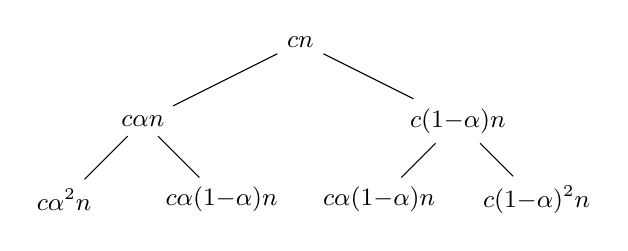
\begin{tikzpicture}[level distance=10mm,
  level 1/.style={sibling distance=40mm},
  level 2/.style={sibling distance=20mm},
  every node/.style={font=\small}]
\node (r) {$cn$}
  child {node {$c\alpha n$}
    child {node {$c\alpha^2n$}}
    child {node {$c\alpha(1{-}\alpha)n$}}}
  child {node {$c(1{-}\alpha)n$}
    child {node {$c\alpha(1{-}\alpha)n$}}
    child {node {$c(1{-}\alpha)^2n$}}};
\end{tikzpicture}\\
{\small Każdy pełny poziom sumuje się do $cn$.}
\end{center}

\formalnie
Niech $\beta=\min(\alpha,1-\alpha)$, $\gamma=\max(\alpha,1-\alpha)$; oba w~$(0,1)$.
Przyjmujemy $T(m)=\Theta(1)$ (między stałymi $d_1,d_2>0$) dla $m\le1$
i~rekurencję dla $m>1$. Węzeł na głębokości $i$ ma rozmiar
$\alpha^{j}(1-\alpha)^{i-j}n\in[\beta^in,\gamma^in]$.

\emph{Dolne oszacowanie.} Dopóki $\beta^in>1$, czyli dla $i<\log_{1/\beta}n$,
żaden węzeł na głębokości $i$ nie jest liściem, więc poziom $i$ jest pełny
i~kosztuje $cn$ (rozmiary na poziomie sumują się do $n$). Zatem
$T(n)\ge cn\floor{\log_{1/\beta}n}=\Omega(n\lg n)$.

\emph{Górne oszacowanie.} Na głębokości $i>\log_{1/\gamma}n$ wszystkie
rozmiary są $<1$, więc drzewo ma $\le\log_{1/\gamma}n+2$ poziomów. Każdy poziom
(także niepełny) kosztuje $\le cn$ w~węzłach wewnętrznych. Liście mają
rozmiar $>\beta$ (ich rodzic miał rozmiar $>1$), a~rozmiary liści sumują się
do $n$, więc liści jest $<n/\beta$ i~kosztują $\O(n)$. Razem
$T(n)\le cn(\log_{1/\gamma}n+2)+d_2n/\beta=\O(n\lg n)$.

\emph{Sprawdzenie metodą podstawiania} (daje też stałą). Niech
$h(\alpha)=-\alpha\lg\alpha-(1-\alpha)\lg(1-\alpha)>0$ (entropia binarna).
Przypuśćmy $T(m)\le Km\lg m$ dla mniejszych argumentów. Wtedy
\begin{align*}
T(n)&\le K\alpha n\lg(\alpha n)+K(1-\alpha)n\lg((1-\alpha)n)+cn\\
&=Kn\lg n-Kn\,h(\alpha)+cn\ \le\ Kn\lg n,
\end{align*}
o ile $K\ge c/h(\alpha)$ (z~odpowiednio dobranym warunkiem brzegowym).

\emph{Sprawdzenie Akrą--Bazzim.} $a_1=a_2=1$, $b_1=\frac1\alpha$, $b_2=\frac1{1-\alpha}$;
$\sum a_ib_i^{-p}=\alpha^p+(1-\alpha)^p=1$ dla $p=1$. Całka: $\int_1^x\frac{cu}{u^2}\,du=c\ln x$, więc
$T(x)=\Theta\bigl(x(1+c\ln x)\bigr)=\Theta(x\lg x)$ \checkmark. Wartość $\alpha$ nie
wpływa na $p$ --- dlatego nierówny podział zmienia tylko stałą.
\begin{odpowiedz}$T(n)=\Theta(n\lg n)$ (asymptotycznie $T(n)\sim\frac{c}{h(\alpha)}\,n\lg n$).\end{odpowiedz}

% ---------------------------------------------------------------------
\section{Zadanie 6. Suma współczynników mniejsza od 1}
\begin{tresc}
Wykaż, że rozwiązanie równania rekurencyjnego
\[
T(n)=\sum_{i=1}^kT(a_in)+n,
\]
gdzie $a_i>0$ dla $i=1,\dots,k$ oraz $\sum_{i=1}^ka_i<1$,
jest postaci $T(n)=\Theta(n)$.
\end{tresc}

\begin{intuicja}
Niech $s=\sum a_i<1$. W~drzewie rekursji suma rozmiarów na poziomie $i$ to
$s^in$ (każdy węzeł rozmiaru $m$ ma dzieci o~łącznym rozmiarze $sm$). Koszty
poziomów tworzą ciąg geometryczny malejący: $n+sn+s^2n+\dots\le\frac{n}{1-s}$.
Już sam korzeń kosztuje $n$, więc $T(n)=\Theta(n)$.
\end{intuicja}
\formalnie
Doprecyzujmy model: $T(n)\in[0,B]$ dla $0<n<n_0$ (warunek brzegowy, $n_0\ge1$
stała), a~dla $n\ge n_0$ obowiązuje rekurencja. Niech $s=\sum a_i<1$,
$\bar a=\max a_i<1$.

\emph{Dolne.} Dla $n\ge n_0$: $T(n)\ge n$, bo $T\ge0$. Zatem $T(n)=\Omega(n)$.

\emph{Górne.} Pokażemy $T(n)\le Kn+B$ dla
$K=\frac{1+(k-1)B}{1-s}$ i~wszystkich $n>0$. Indukcja po $j$: teza $P_j$ ---
nierówność zachodzi dla $n<n_0/\bar a^{\,j}$.
$P_0$: dla $n<n_0$ mamy $T(n)\le B$ \checkmark. $P_j\Rightarrow P_{j+1}$: dla
$n_0\le n<n_0/\bar a^{\,j+1}$ wszystkie $a_in<n_0/\bar a^{\,j}$, więc
\[
T(n)\le\sum_{i=1}^k(Ka_in+B)+n = Ksn+kB+n.
\]
Chcemy $Ksn+kB+n\le Kn+B$, tj.\ $n\bigl(K(1-s)-1\bigr)\ge(k-1)B$. Z~wyboru $K$
lewa strona to $n(k-1)B\ge(k-1)B$, bo $n\ge n_0\ge1$ \checkmark.
Każde $n$ jest objęte pewnym $P_j$, więc $T(n)\le Kn+B=\O(n)$.

\emph{Sprawdzenie Akrą--Bazzim.} Wszystkie wagi w~(A--B) są równe 1,
a~dzielniki to $b_i=1/a_i>1$, więc $\varphi(q)=\sum_ia_i^{\,q}$.
Ponieważ $\varphi(1)=\sum a_i<1$, mamy $p<1$; ponadto $\varphi(0)=k\ge1$,
więc $p\ge0$. Całka:
\[
\int_1^x\frac{u}{u^{p+1}}\,du=\int_1^xu^{-p}\,du=\frac{x^{1-p}-1}{1-p}=\Theta(x^{1-p}),
\]
więc $T(x)=\Theta\bigl(x^p\cdot x^{1-p}\bigr)=\Theta(x)$ \checkmark. Zatem
$\sum a_i<1$ to dokładnie warunek $p<1$, przy którym dominuje korzeń.
\begin{odpowiedz}$n\le T(n)\le\frac{1+(k-1)B}{1-\sum a_i}\,n+B$, czyli $T(n)=\Theta(n)$.\end{odpowiedz}

\begin{uwaga}
Gdy $\sum a_i=1$ (jak w~zad.~5), poziomy kosztują po tyle samo i~wychodzi
$\Theta(n\lg n)$; gdy $\sum a_i>1$ --- dominują liście i~wynik jest
wielomianowo większy od $n$.
\end{uwaga}

% ---------------------------------------------------------------------
\section{Zadanie 7. Rekurencje z sufitami}
\begin{tresc}
Rozwiąż z~dokładnością do $\Theta$ równania:
\begin{enumerate}[label=(\alph*)]
\item $T(n)=T(\ceil{n/5})+T(\ceil{7n/10})+\Theta(n)$,
\item $T(n)=T(\ceil{n/5})+T(\ceil{3n/4})+\Theta(n)$.
\end{enumerate}
\end{tresc}

\begin{intuicja}
(a) to rekurencja algorytmu \textbf{magicznych piątek} (wybór $k$-tego
elementu w~czasie liniowym, \emph{median of medians}): rekurencja na
$n/5$ medianach grup i~na co najwyżej $\approx7n/10$ elementach. Ponieważ
$\frac15+\frac7{10}=\frac9{10}<1$, z~zadania 6 spodziewamy się $\Theta(n)$.
W~(b) $\frac15+\frac34=\frac{19}{20}<1$ --- też $\Theta(n)$. Jedyna nowość to
sufity: $\ceil{x}\le x+1$, czyli każdy sufit dokłada stałą, którą
„połykamy”, biorąc $n$ dostatecznie duże.
\end{intuicja}
\formalnie
Niech składnik $\Theta(n)$ to $g(n)$ z~$c_1n\le g(n)\le c_2n$, a~$T(n)>0$
dla małych $n$ (warunek brzegowy).

\emph{Dolne} (oba przypadki): $T(n)\ge g(n)\ge c_1n$.

\emph{Górne (a).} Pokażemy $T(n)\le Kn$ dla $n\ge1$, gdzie
$K=\max\bigl(20c_2,\ \max_{n<40}T(n)/n\bigr)$. Dla $n<40$ z~wyboru $K$.
Dla $n\ge40$ argumenty $\ceil{n/5},\ceil{7n/10}$ są mniejsze od $n$, więc
z~założenia indukcyjnego i~$\ceil x\le x+1$:
\begin{align*}
T(n)&\le K\Bigl(\frac n5+1\Bigr)+K\Bigl(\frac{7n}{10}+1\Bigr)+c_2n\\
&=Kn-\Bigl(\frac{Kn}{10}-c_2n-2K\Bigr).
\end{align*}
Ponieważ $K\ge20c_2$, mamy $\frac{Kn}{10}-c_2n\ge\frac{Kn}{20}\ge2K$ dla $n\ge40$, więc nawias
jest $\ge0$ i~$T(n)\le Kn$ \checkmark.

\emph{Górne (b).} Identycznie z~$K=\max\bigl(40c_2,\max_{n<80}T(n)/n\bigr)$:
\[
T(n)\le K\Bigl(\frac n5+1\Bigr)+K\Bigl(\frac{3n}4+1\Bigr)+c_2n=Kn-\Bigl(\frac{Kn}{20}-c_2n-2K\Bigr),
\]
a $\frac{Kn}{20}-c_2n\ge\frac{Kn}{40}\ge2K$ dla $n\ge80$.

\emph{Sprawdzenie Akrą--Bazzim.} Składnik $\Theta(n)$ rośnie wielomianowo
(Fakt~\ref{fakt:wielom}), więc sufity można pominąć
(Tw.~\ref{tw:akra-sufity}; to też zaburzenia $|h_i(n)|<1$ z~Faktu~\ref{fakt:akra-h}).
(a) to przykład z~wykładu: $(1/5)^p+(7/10)^p=1$ daje $p\approx0{,}840$; (b)
$(1/5)^p+(3/4)^p=1$ daje $p\approx0{,}911$. W~obu przypadkach $p<1$, bo
$\varphi(1)<1$. Jak w~zad.~6 dostajemy $T(n)=\Theta(n^p\cdot n^{1-p})=\Theta(n)$ \checkmark.
\begin{odpowiedz}(a) $T(n)=\Theta(n)$;\quad (b) $T(n)=\Theta(n)$.\end{odpowiedz}

% ---------------------------------------------------------------------
\section{Zadanie 8. \texorpdfstring{$T(n)=T(\ceil{\log n})+1/\log^*n$}{T(n) = T(ceil(log n)) + 1/log* n}}
\begin{tresc}
Rozwiąż z~dokładnością do $\Theta$ równanie
$T(n)=T(\ceil{\log n})+\dfrac{1}{\log^*n}$, $T(n)=0$ $(n\le2)$.
\end{tresc}
Przyjmujemy $\log=\lg$ (dla innej stałej podstawy wynik jest taki sam).

\begin{teoria}[Wieże potęg]
$\mathrm{tow}(0)=1$, $\mathrm{tow}(k)=2^{\mathrm{tow}(k-1)}$: $1,2,4,16,65536,\dots$
Z~definicji $\lgs$ (zestaw 0): $\lgs x=k\iff \mathrm{tow}(k-1)<x\le\mathrm{tow}(k)$ dla $k\ge1$.
\end{teoria}

\begin{intuicja}
Każde wywołanie logarytmuje argument, więc wywołań jest ok.\ $\lgs n$.
W~wywołaniu numer $i$ (licząc od $0$) argument ma $\lgs$ równe $\lgs n-i$,
więc dodajemy $\frac{1}{\lgs n},\frac1{\lgs n-1},\dots,\frac12$ --- to jest
liczba harmoniczna! $T(n)\approx H_{\lgs n}\approx\ln\lgs n$.
\end{intuicja}

\begin{lemat}
Dla całkowitego $m>1$: $\lgs\ceil{\lg m}=\lgs m-1$.
\end{lemat}
\begin{proof}
Niech $k=\lgs m\ge1$, czyli $\mathrm{tow}(k-1)<m\le\mathrm{tow}(k)$. Logarytmując:
$\mathrm{tow}(k-2)<\lg m\le\mathrm{tow}(k-1)$ (dla $k=1$ czytamy lewą stronę jako
$\lg m>0$). Ponieważ $\mathrm{tow}(k-1)$ jest całkowite, także
$\ceil{\lg m}\le\mathrm{tow}(k-1)$, a $\ceil{\lg m}\ge\lg m$. Zatem $\ceil{\lg m}$
leży w~tym samym przedziale co $\lg m$, czyli $\lgs\ceil{\lg m}=\lgs(\lg m)=k-1$
(dla $k=1$: $m=2$, $\ceil{\lg2}=1$, $\lgs1=0$ \checkmark).
\end{proof}

\formalnie
Niech $n\ge3$, $L=\lgs n\ge2$ i~$n_0=n$, $n_{i+1}=\ceil{\lg n_i}$. Z~lematu
$\lgs n_i=L-i$. Rekurencja zatrzymuje się przy pierwszym $n_t\le2$, tzn.\
$\lgs n_t\le1$, czyli przy $t=L-1$. Zatem
\[
T(n)=\sum_{i=0}^{L-2}\frac{1}{\lgs n_i}=\sum_{i=0}^{L-2}\frac{1}{L-i}=\sum_{j=2}^{L}\frac1j=H_{L}-1.
\]
Z~zad.~6 zestawu 0: $\ln L<H_L<\ln L+1$, więc $T(n)=\Theta(\lg L)$.
Sprawdzenie: $T(3)=T(2)+\frac{1}{\lgs3}=\frac12=H_2-1$ \checkmark.

\begin{uwaga}
Tu też nie ma zastosowania ani Master Theorem, ani Akra--Bazzi: argument
spada z~$n$ do $\lg n$, a nie do $b\cdot n$.
\end{uwaga}
\begin{odpowiedz}$T(n)=H_{\lgs n}-1=\Theta(\lg\lgs n)$ dla $n\ge3$.\end{odpowiedz}

% ---------------------------------------------------------------------
\section{Zadanie 9. Warunek regularności}
\begin{tresc}
Pokaż, że warunek regularności (w~twierdzeniu o~rekurencji uniwersalnej)
$af(n/b)\le cf(n)$ dla pewnej stałej $c<1$ implikuje, że istnieje stała
$\varepsilon>0$, taka że $f(n)=\Omega(n^{\log_ba+\varepsilon})$.
\end{tresc}

\begin{intuicja}
Warunek mówi: $f(n)\ge\frac ac f(n/b)$ --- gdy argument rośnie $b$ razy,
wartość rośnie co najmniej $\frac ac$ razy. Funkcja $n^{p}$ rośnie dokładnie
$b^p$ razy. Zatem $f$ zachowuje się co najmniej jak $n^{q}$ z~$b^q=\frac ac$,
tj.\ $q=\log_b\frac ac=\log_ba+\log_b\frac1c$. Ponieważ $c<1$, nadwyżka
$\varepsilon=\log_b\frac1c$ jest dodatnia. Dlatego w~przypadku 3 warunek
regularności „zawiera” założenie $f=\Omega(n^{p+\varepsilon})$
(Uwaga 2 z~wykładu).
\end{intuicja}
\formalnie
Założenia: $a\ge1$, $b>1$, $0<c<1$; nierówność $af(n/b)\le cf(n)$ zachodzi dla
wszystkich $n\ge n_0$ (z~$n_0\ge b$), a~$f$ jest dodatnia i~ograniczona z~dołu
przez $\delta>0$ na przedziale $[n_0,bn_0)$ (tak jest np.\ dla $f$ niemalejącej
lub ciągłej i~dodatniej --- „rozsądne” $f$ z~analizy algorytmów).

Niech $n\ge n_0$. Istnieją jednoznacznie $j\ge0$ i~$x\in[n_0,bn_0)$ takie, że
$n=b^jx$. Stosując warunek $j$ razy w~punktach $b^jx,b^{j-1}x,\dots,bx$ (wszystkie
$\ge n_0$):
\begin{align*}
f(n)&\ge \frac ac\,f\Bigl(\frac nb\Bigr)\ \ge\ \Bigl(\frac ac\Bigr)^2f\Bigl(\frac n{b^2}\Bigr)\ \ge\ \dots\\
&\ge \Bigl(\frac ac\Bigr)^jf(x)\ \ge\ \Bigl(\frac ac\Bigr)^j\delta.
\end{align*}
Niech $\varepsilon=\log_b\frac1c>0$. Wtedy $\frac ac=b^{\log_ba+\varepsilon}$, więc
\[
\Bigl(\frac ac\Bigr)^j=\bigl(b^j\bigr)^{\log_ba+\varepsilon}=\Bigl(\frac nx\Bigr)^{\log_ba+\varepsilon}
\ge\Bigl(\frac{n}{bn_0}\Bigr)^{\log_ba+\varepsilon}.
\]
Zatem $f(n)\ge\delta(bn_0)^{-(\log_ba+\varepsilon)}\cdot n^{\log_ba+\varepsilon}$
dla $n\ge n_0$, czyli $f(n)=\Omega(n^{\log_ba+\varepsilon})$.\qed

\begin{uwaga}[Implikacja odwrotna nie zachodzi]
Dla $a=1$, $b=2$ weźmy $f(n)=4^{\ceil{\log_4n}}$. Mamy $n\le f(n)<4n$, więc
$f(n)=\Omega(n^{0+1})$. Ale dla $n=4^k$: $f(n/2)=4^{\ceil{k-1/2}}=4^k=f(n)$,
więc $af(n/2)\le cf(n)$ z~$c<1$ nie zachodzi dla nieskończenie wielu $n$.
\end{uwaga}
\begin{odpowiedz}
Z~regularności $f(n)=\Omega\bigl(n^{\log_ba+\varepsilon}\bigr)$ dla $\varepsilon=\log_b(1/c)>0$.
\end{odpowiedz}

% ---------------------------------------------------------------------
\section{Zadanie 10. Maksymalna suma spójnego fragmentu}
\begin{tresc}
Zaproponuj algorytm „dziel i zwyciężaj”, który dla zadanej tablicy $A$
o~rozmiarze $n$ zawierającej liczby całkowite znajduje indeksy $i$ oraz $j$
maksymalizujące sumę $A[i]+A[i+1]+A[i+2]+\ldots+A[j]$.
Wykaż poprawność tego algorytmu i~przeanalizuj liczbę wykonywanych przez niego porównań.
\end{tresc}

\begin{intuicja}
Przetnij tablicę na pół. Najlepszy fragment albo leży całkowicie w~lewej
połowie, albo całkowicie w~prawej, albo \emph{przecina środek}. Dwa pierwsze
przypadki załatwia rekurencja. Fragment przecinający środek to „jakiś
sufiks lewej połowy” + „jakiś prefiks prawej połowy”, a~te dwie części
wybieramy \emph{niezależnie}: najlepszy sufiks (idąc od środka w~lewo)
i~najlepszy prefiks (od środka w~prawo). To jest liniowe. Daje to
$T(n)=2T(n/2)+\Theta(n)=\Theta(n\lg n)$, jak mergesort.
\end{intuicja}

Zakładamy, że szukamy fragmentu niepustego ($i\le j$); indeksujemy $1..n$,
$S(i,j)=\sum_{t=i}^jA[t]$.

\begin{algorithm}[H]
\caption{\textsc{MaxFrag}$(A,l,r)$ --- zwraca $(i,j,S(i,j))$ maksymalne dla $l\le i\le j\le r$}
\begin{algorithmic}[1]
\If{$l=r$} \Return $(l,l,A[l])$ \EndIf
\State $m\gets\floor{(l+r)/2}$
\State $L\gets$ \Call{MaxFrag}{$A,l,m$};\quad $R\gets$ \Call{MaxFrag}{$A,m+1,r$}
\Statex \(\triangleright\) najlepszy sufiks lewej połowy $A[i..m]$
\State $s\gets A[m]$;\ $\mathit{best}_L\gets s$;\ $i\gets m$
\For{$t\gets m-1$ \textbf{w dół do} $l$}
  \State $s\gets s+A[t]$
  \If{$s>\mathit{best}_L$} $\mathit{best}_L\gets s$;\ $i\gets t$ \EndIf
\EndFor
\Statex \(\triangleright\) najlepszy prefiks prawej połowy $A[m{+}1..j]$
\State $s\gets A[m+1]$;\ $\mathit{best}_R\gets s$;\ $j\gets m+1$
\For{$t\gets m+2$ \textbf{do} $r$}
  \State $s\gets s+A[t]$
  \If{$s>\mathit{best}_R$} $\mathit{best}_R\gets s$;\ $j\gets t$ \EndIf
\EndFor
\State $X\gets(i,j,\mathit{best}_L+\mathit{best}_R)$
\State \Return ten z~$L,R,X$, który ma największą sumę (2~porównania)
\end{algorithmic}
\end{algorithm}

\textbf{Poprawność.} Indukcja po długości $r-l+1$. Dla jednego elementu
jedyny fragment to $[l,l]$ \checkmark. Dla $l<r$ każdy fragment $[i',j']$
spełnia dokładnie jeden z~warunków:
\begin{enumerate}
\item $j'\le m$ --- wtedy $S(i',j')\le$ suma w~$L$ (zał.\ indukcyjne);
\item $i'\ge m+1$ --- wtedy $S(i',j')\le$ suma w~$R$;
\item $i'\le m<j'$ --- wtedy $S(i',j')=S(i',m)+S(m+1,j')$. Pętle przeglądają
\emph{wszystkie} $i'\in[l,m]$ i~\emph{wszystkie} $j'\in[m+1,r]$, więc
$\mathit{best}_L=\max_{i'}S(i',m)$, $\mathit{best}_R=\max_{j'}S(m+1,j')$.
Ponieważ oba składniki są niezależne,
$\max_{i',j'}\bigl(S(i',m)+S(m+1,j')\bigr)=\mathit{best}_L+\mathit{best}_R$,
czyli $S(i',j')\le$ suma w~$X$.
\end{enumerate}
Zwracamy maksimum z~$L,R,X$; każdy z~nich jest prawdziwym fragmentem
$[l,r]$, a~każdy fragment ma sumę $\le$ jednego z~nich --- więc wynik jest
optymalny.\qed

\textbf{Liczba porównań.} Liczymy porównania sum (instrukcje \textbf{if} i~wybór
maksimum). Lewa połowa ma $\ceil{n/2}$ elementów: pętla to $\ceil{n/2}-1$
porównań; prawa: $\floor{n/2}-1$; wybór maksimum z~trzech: 2. Razem
$n$ porównań poza rekurencją:
\[
P(1)=0,\qquad P(n)=P(\ceil{n/2})+P(\floor{n/2})+n\quad(n\ge2).
\]
To prawie rekurencja z~zad.~9 zestawu 0 ($C_n$ z~„$+n-1$”). Niech $Q(n)=P(n)-(n-1)$:
\[
Q(n)=Q(\ceil{n/2})+Q(\floor{n/2})+n-1,\quad Q(1)=0,
\]
bo $P(n)-(n-1)=Q(\ceil{n/2})+\bigl(\ceil{n/2}-1\bigr)+Q(\floor{n/2})+\bigl(\floor{n/2}-1\bigr)+n-(n-1)$,
a~wyrazy wolne sumują się do $n-2+1=n-1$. Zatem $Q(n)=C_n=n\ceil{\lg n}+1-2^{\ceil{\lg n}}$ i
\[
P(n)=n\ceil{\lg n}+n-2^{\ceil{\lg n}}.
\]
Dla $n=2^k$: $P(n)=nk=n\lg n$. (Wzór sprawdzony programem dla $n\le120$.)
\begin{odpowiedz}
Algorytm wykonuje $P(n)=n\ceil{\lg n}+n-2^{\ceil{\lg n}}=\Theta(n\lg n)$ porównań
(dokładnie $n\lg n$ dla $n$ będącego potęgą dwójki).
\end{odpowiedz}

\begin{uwaga}
Problem da się rozwiązać w~czasie $\Theta(n)$ algorytmem Kadane
(programowanie dynamiczne): jeśli $E_t$ to największa suma fragmentu
kończącego się na pozycji $t$, to $E_t=\max(A[t],\,E_{t-1}+A[t])$, a~wynik
to $\max_tE_t$. Również
dziel i~zwyciężaj można przyspieszyć do $\Theta(n)$, jeśli rekurencja
zwraca dodatkowo sumę całości, najlepszy prefiks i~najlepszy sufiks
--- wtedy krok łączenia jest stały: $T(n)=2T(n/2)+\Theta(1)$.
\end{uwaga}

\end{document}
